\documentclass{beamer}

\newcommand\SSys{\ensuremath{S_{\text{sys}}}}
\newcommand\SEnv{\ensuremath{S_{\text{env}}}}
\newcommand\STot{\ensuremath{S_{\text{tot}}}}

% Environments

% Math
\newcommand{\Equation}[1]{\begin{equation*}#1\end{equation*}}    % equation
\newcommand{\NEquation}[1]{\begin{equation}#1\end{equation}}     % equation (numbered)
\newcommand{\Align}[1]{\begin{align*}#1\end{align*}}             % block equation without numbering
\newcommand{\NAlign}[1]{\begin{align}#1\end{align}}              % block equation with numbering. Use \notag to suppress numbering locally.
%\newcommand{\Inline}[1]{\(#1\)}                                  % inline equation DEPRECATED.
% Sub-math
\newcommand{\Split}[1]{\begin{split}#1\end{split}}               % split (for use inside Align)
\newcommand{\Cases}[1]{\begin{cases}#1\end{cases}}               % piecewise functions etc (for use in math mode)
% Matrices
\newcommand{\Matrix}[1]{\begin{matrix}#1\end{matrix}}            % matrix without parentheses
\newcommand{\MatrixP}[1]{\begin{pmatrix}#1\end{pmatrix}}         % () matrix ("parentheses matrix")
\newcommand{\MatrixB}[1]{\begin{bmatrix}#1\end{bmatrix}}         % [] matrix ("braces matrix")
\newcommand{\MatrixC}[1]{\begin{Bmatrix}#1\end{Bmatrix}}         % {} matrix ("curly matrix")
\newcommand{\MatrixD}[1]{\begin{vmatrix}#1\end{vmatrix}}         % || matrix ("det matrix")
\newcommand{\MatrixN}[1]{\begin{Vmatrix}#1\end{Vmatrix}}         % || || matrix ("norm matrix")
% Quotes
\newcommand{\Qe}[1]{`#1'}                                        % quotes english
\newcommand{\Dqe}[1]{``#1''}                                     % double quotes english
\newcommand{\Qg}[1]{\glq{}#1\grq}                                % quotes german
\newcommand{\Dqg}[1]{\glqq{}#1\grqq}                             % double quotes german



% Abbreviations for common operations

% General
\renewcommand{\d}{\mathrm{d}}                                    % differential
\renewcommand{\i}{\mathrm{i}}                                    % imaginary unit
\renewcommand{\inf}{\infty}                                      % infinity
\newcommand{\infint}{\int_{-\inf}^\inf}                          % integral from -inf to inf
\newcommand{\inflint}{\int\limits_{-\inf}^\inf}                  % integral from -inf to inf with \limits
% Differential quotients
\newcommand{\tdq}[2]{\frac{\d #1}{\d #2}}                        % total differential quotient
\newcommand{\pdq}[2]{\frac{\partial #1}{\partial #2}}            % partial differential quotient
\newcommand{\vpdq}[1]{\frac{\vec\partial}{\vec\partial #1}}      % vector partial differential quotient
\newcommand{\vdq}[2]{\frac{\delta #1}{\delta #2}}                % variational differential quotient
% Frequent terms
\renewcommand\exp{\operatorname{exp}}                            % exp
\renewcommand\sin{\operatorname{sin}}                            % sin
\renewcommand\cos{\operatorname{cos}}                            % cos
\renewcommand\tan{\operatorname{tan}}                            % tan
\renewcommand\cot{\operatorname{cot}}                            % cot
\renewcommand\Re{\operatorname{Re}}                              % Re
\renewcommand\Im{\operatorname{Im}}                              % Im
\newcommand\Res{\operatorname*{Res}}                             % Res (* produces underset subscripts)
\renewcommand\div{\operatorname{div}}                            % div
\newcommand\grad{\operatorname{grad}}                            % grad
\newcommand\curl{\operatorname{curl}}                            % curl
\newcommand\rot{\operatorname{curl}}                             % rot = curl
\newcommand\sign{\operatorname{sign}}                            % sign
\renewcommand\deg{\operatorname{deg}}                            % degree
\newcommand\supp{\operatorname{supp}}                            % support
\newcommand\Tr{\operatorname{Tr}}                                % trace
\renewcommand\det{\operatorname{det}}                            % determinant
\newcommand\ind{\operatorname{ind}}                              % winding number
\newcommand\vol{\operatorname{vol}}                              % volume form
\newcommand\unity{\mathds{1}}                                    % identity matrix/operator
\newcommand\id{\operatorname{Id}}                                % identity
\newcommand\const{\mathrm{const.}}                               % Constants



% Redefinitions, fixing ambiguities
\newcommand\hodge{*}                                             % Hodge star
\newcommand\cross{\times}                                        % cross product
\renewcommand\vec[1]{\boldsymbol{#1}}                            % print vectors bold
\newcommand\laplace{\Delta}                                      % Laplace operator



% Special fonts
\newcommand\Cal[1]{\mathcal{#1}}                                 % Calligraphic (upper/lower case)
\newcommand\Frak[1]{\mathfrak{#1}}                               % Fraktur (upper/lower case)
\newcommand\Script[1]{\mathscr{#1}}                              % Script (upper case only)
\newcommand\Set[1]{\mathbb{#1}}                                  % Set/double stroke (upper case only)



% Units (m/s^2)
\newcommand{\Unit}[1]{\;\mathrm{#1}}



% References to different objects
\newcommand{\RefTheorem}[1]{\hyperref[#1]{\{\ref*{#1}\}}} % {123}
\newcommand{\RefEqn}[1]{\hyperref[#1]{(\ref*{#1})}} % (123)
\newcommand{\RefFigure}[1]{\hyperref[#1]{\ref*{#1}}} % 123
\newcommand{\RefSection}[1]{\hyperref[#1]{\ref*{#1}}} % 123



% Nicer square root
\def\nicesqrt{\mathpalette\DHLhksqrt}
\def\DHLhksqrt#1#2{%
\setbox0=\hbox{$#1\oldsqrt{#2\,}$}\dimen0=\ht0%
\advance\dimen0-0.2\ht0%
\setbox2=\hbox{\vrule height\ht0 depth -\dimen0}%
{\box0\lower0.4pt\box2}}































% AMS packages
\usepackage{amsmath, amssymb, amstext}



% Tensor package
% Full documentation: http://ftp.uni-erlangen.de/mirrors/CTAN/macros/latex/contrib/tensor/tensor.pdf
% Usage:
% Indices only: \indices{^a_{bc}}
% Tensor: \tensor[indices before]{tensor name}{indices after}
\usepackage{tensor}



% smashoperator
\usepackage{mathtools}



% Provides better support for underlined (etc) text. Use [normalem] to not alter \emph to underlining.
\usepackage[normalem]{ulem}



% Cancel package (strike-through formulas)
% Usage: \cancel{} \bcancel{} \xcancel{} \cancelto{}{}
\usepackage{cancel}



% Extended graphics support
\usepackage{graphicx}



% Colorizing things
% Usage: {\color{grey}lorem ipsum}
\usepackage{xcolor}
\definecolor{gray}{rgb}{0.6,0.6,0.6}
\definecolor{red}{rgb}{0.8,0,0}
\definecolor{green}{rgb}{0.04,0.62,0.14}
% Mathematica's first four ColorData[1] colors:
\definecolor{mathematica1}{rgb}{0.2472, 0.24, 0.6}
\definecolor{mathematica2}{rgb}{0.6, 0.24, 0.442893}
\definecolor{mathematica3}{rgb}{0.6, 0.547014, 0.24}
\definecolor{mathematica4}{rgb}{0.24, 0.6, 0.33692}
% Todo placeholder:
\newcommand{\Todo}[1]{{\color{red}[TODO: #1]}}



% Double strike font \mathds{}
\usepackage{dsfont}



% Script font \mathscr{}
\usepackage{mathrsfs}



% Hyperlinks, internal and external.
\usepackage{hyperref}
% \hypersetup{
% 	% Color links
% 	colorlinks=true,
% 	citecolor=black,
% 	filecolor=black,
% 	linkcolor=black,
% 	urlcolor=black
% }



% Create index.
% Create entry via \index{name[subname[subsubname]] (depth optional)
% Print using \printindex
\usepackage{makeidx} \makeindex



% Generate warnings when using deprecated commands
\usepackage[l2tabu, orthodox]{nag}



% Multicolumn sections.
% Example: Two-column layout: \begin{multicols}{2} lorem ipsum \end{multicols}
\usepackage{multicol}

% Enables lipsum text using \lipsum. \lipsum[i-j] prints paragraphs i to j. Maximum is 150.
\usepackage{lipsum}
\setlipsumdefault{1} % Print first paragraph by default



% Better date/time support
\usepackage{datetime}
\renewcommand{\dateseparator}{-}
\renewcommand{\timeseparator}{:}
\newcommand\Date{\the\year \dateseparator \twodigit\month \dateseparator \twodigit\day}
\newcommand\Time{\currenttime}







































% TikZ
\usepackage{tikz}
\usetikzlibrary{
	arrows,
	backgrounds,
	calc,
	decorations.markings,
	decorations.pathmorphing,
	fit,
	intersections,
	patterns,
	positioning,
	through
}

% Arc around a point
\newcommand\TikzArcAround[3]{
	% #1: radius
	% #2: start angle
	% #3: delta angle
	% Example: \draw (1,0) \ArcAround{2}{60}{120}
	++(#2:#1)
	arc[radius=#1, start angle=#2, delta angle=#3]
}

% Helper coordinate system
\newcommand\TikzCoSy[4]{
	% Arguments: integers: x1, x2, y1, y2 ("x range, y range")
	% Lower numbers first!
	(#1,#3) grid (#2,#4)
}
\newcommand\TikzCoSyLabels[4] {
	\foreach \x in {#1,...,#2} {
		node at (\x,0) {\x}
	}
	\foreach \y in {#3,...,#4} {
		\ifnum \y = 0
		\else
			node at (0,\y) {\y}
		\fi
	}
}
\newcommand\TikzFullCoSy[4] {
	\TikzCoSy{#1}{#2}{#3}{#4}
	\TikzCoSyLabels{#1}{#2}{#3}{#4}
}

% Draws a cross at the current location with radius #1.
\newcommand\TikzCross[1]{
	% 0.707107/2 = 1/sqrt(2) for the rotation to get the "x" shape
	+( #1/0.707107/2, #1/0.707107/2) -- +(-#1/0.707107/2,-#1/0.707107/2)
	+( #1/0.707107/2,-#1/0.707107/2) -- +(-#1/0.707107/2, #1/0.707107/2)
	+(0,0)
}

\newcommand\TikzClipMask{
	\draw [draw=black, fill=orange, opacity=0.5, draw opacity=0.8]
}

% Useful for decorations.
% Example:
% mark=between positions 0.0 and 1.0 step 0.1 with {\node (node\pgfkeysvalueof{\SequenceNumber}) [label=below right:{$y_\pgfkeysvalueof{\SequenceNumber}$}] {};}
% Adds nodes named "nodeX" at evenly spaced intervals to a path.
\newcommand\SequenceIndex{\pgfkeysvalueof{/pgf/decoration/mark info/sequence number}}

% Parse mathematical expressions
\newcommand\TikzMath[1] {
	\pgfmathparse{#1}
	\pgfmathresult
}

% Use stealth arrowheads as default
\tikzstyle{every picture}+=[>=stealth]


% Draw arrow at arbitrary position using ->-=0.5 etc
\tikzset{->-/.style={decoration={
	markings,
	mark=at position #1 with {\arrow{>}}},postaction={decorate}}}














\mode<presentation>
{
  \usetheme{boxes}
  \setbeamercovered{transparent}
}


\usepackage[english]{babel}
\usepackage[latin1]{inputenc}
\usepackage{times}
\usepackage[T1]{fontenc}
% Or whatever. Note that the encoding and the font should match. If T1
% does not look nice, try deleting the line with the fontenc.


% \title[Short Paper Title] % (optional, use only with long paper titles)
% {Title As It Is In the Proceedings}
\title{Entropy in continuous phase space}

%\subtitle{Include Only If Paper Has a Subtitle}

\author{David Luposchainsky}

\institute[University of W�rzburg]{
	University of W�rzburg, Institute of Theoretical Physics 3
}

\date{Group seminar presentation}

\subject{Entropy}
% This is only inserted into the PDF information catalog. Can be left
% out.



% If you have a file called "university-logo-filename.xxx", where xxx
% is a graphic format that can be processed by latex or pdflatex,
% resp., then you can add a logo as follows:

% \pgfdeclareimage[height=0.5cm]{university-logo}{university-logo-filename}
% \logo{\pgfuseimage{university-logo}}



% Delete this, if you do not want the table of contents to pop up at
% the beginning of each subsection:
% \AtBeginSubsection[]
% {
%   \begin{frame}<beamer>{Outline}
%     \tableofcontents[currentsection,currentsubsection]
%   \end{frame}
% }


% If you wish to uncover everything in a step-wise fashion, uncomment
% the following command:

%\beamerdefaultoverlayspecification{<+->}


\begin{document}

\begin{frame}
	\titlepage
\end{frame}

% \begin{frame}{Outline}
%   \tableofcontents
%   % You might wish to add the option [pausesections]
% \end{frame}


\section{Introduction}

\subsection{Basic entropy-producing processes}

\begin{frame}
	\frametitle{Entropy-producing processes of interest}
	\begin{itemize}
		\item Discrete: Markov jump processes. Spontaneous transitions between discrete configurations \(c\in\Omega\) with rates \(w_{c\to c'}\)
		\item Continuous, overdamped -- ``no momentum'' following a DE of the form
			\Align{
				\dot q = F(q) + \Gamma(q)\xi(t)
			}
		\item Continuous, underdamped -- full phase space required, e.g.
			\Align{
				\dot q &= p \\
				\dot p &= F(q) -\gamma(p)p+ \Gamma(p)\xi(t)
			}
	\end{itemize}
\end{frame}


\begin{frame}
	\frametitle{Last time: Discrete systems}
	\begin{itemize}
		\item Set of discrete microstates \(c\in\Omega\)
		\item Continuous time
		\item Transitions between the microstates at transition rates \(w_{c\to c'}\)
	\end{itemize}
\end{frame}



\begin{frame}
	\frametitle{Stochastic trajectories}
	The evolution of a system looks like
	\vspace{-2em}
	\begin{figure}[htb]
		\centering
		\begin{tikzpicture}
	[>=stealth, scale=.5]

	% coordinate system
	\begin{scope}
		% axes
		\begin{scope}[->]
			\newcommand\Excess{0.2}
			\draw (-\Excess,0) -- (10.5,0); % x
			\draw (0,-\Excess) -- (0,6);  % y
		\end{scope}


		\newcommand{\TickLength}{0.2}
		\newcommand{\LabelOffset}{0.5}
		
		% y axis labels/ticks
		\begin{scope}
			\foreach \y in {1,...,5} {
				\draw (-\TickLength/2, \y) -- (\TickLength/2, \y);
 				\node at (-\LabelOffset, \y) {\(\y\)};
			}
			\node at (0, 6 + \LabelOffset) {\(n\)};
		\end{scope}

		% x axis labels/ticks
		\begin{scope}
			\foreach \i/\x in {0/0, 1/2, 2/3, 3/6, 4/7.5, 5/8, 6/10} {
				\draw (\x, -\TickLength/2) -- (\x, \TickLength/2);
				\node at (\x, -\LabelOffset) {\(\tau_\i\)};
			}
			\node at (0, -2*\LabelOffset) {\(0\)};
			\node at (10, -2*\LabelOffset) {\(T\)};

			\node at (10.5 + \LabelOffset, 0) {\(t\)};
		\end{scope}

	\end{scope}

	% Path taken
	\begin{scope}
		
		% Actual path
		\begin{scope} [thick]
			\draw (0,1) -- (2,1)
				(2,4) -- (3,4)
				(3,3) -- (6,3)
				(6,5) -- (7.5,5)
				(7.5,1) -- (8,1)
				(8,2) -- (10,2)
				;
			\newcommand{\Radius}{0.03}
			\foreach \xy in {(0,1), (2,1), (2,4), (3,4), (3,3), (6,3), (6,5), (7.5,5), (7.5,1), (8,1), (8,2), (10,2)} {
				\draw[fill=black] \xy circle (\Radius);
			}
		\end{scope}

		% Connecting jump lines
		\begin{scope} [dotted]
			\draw (2,1)-- (2,4)
			      (3,4) -- (3,3) 
				(6,3) -- (6,5) 
				(7.5,5) -- (7.5,1) 
				(8,1) -- (8,2)
				;
		\end{scope}

		% labels
% 		\begin{scope}
% 			\newcommand{\LabelOffset}{0.5}
% 			\node at (0.5,       1 - 0.5*\LabelOffset) {\tiny \(n_0^+ \!\! = \! 1\)}; % tau 0
% 			\node at (2,         1 - 0.5*\LabelOffset) {\tiny \(n_1^- \!\! = \! 1\)}; % tau 1
% 			\node at (2,         4 + 0.5*\LabelOffset) {\tiny \(n_1^+ \!\! = \! 4\)};
% 			\node at (3,         4 + 0.5*\LabelOffset) {\tiny \(n_2^- \!\! = \! 4\)}; % tau 2
% 			\node at (3,         3 - 0.5*\LabelOffset) {\tiny \(n_2^+ \!\! = \! 3\)};
% 			\node at (6,         3 - 0.5*\LabelOffset) {\tiny \(n_3^- \!\! = \! 3\)}; % tau 3
% 			\node at (6,         5 + 0.5*\LabelOffset) {\tiny \(n_3^+ \!\! = \! 5\)};
% 			\node at (7.5,       5 + 0.5*\LabelOffset) {\tiny \(n_4^- \!\! = \! 5\)}; % tau 4
% 			\node at (7.5 - 0.2, 1 - 0.5*\LabelOffset) {\tiny \(n_4^+ \!\! = \! 1\)};
% 			\node at (8 + 0.2,   1 - 0.5*\LabelOffset) {\tiny \(n_5^- \!\! = \! 1\)}; % tau 5
% 			\node at (8,         2 + 0.5*\LabelOffset) {\tiny \(n_5^+ \!\! = \! 2\)};
% 			\node at (10-0.5,    2 + 0.5*\LabelOffset) {\tiny \(n_6^- \!\! = \! 2\)}; % tau 6
% 		\end{scope}

		% final dashed line at t=T

		\begin{scope}
			\draw [dashed] (10,0) -- (10,6);
		\end{scope}
		
	\end{scope}

\end{tikzpicture}

	\end{figure}
	\vspace{-2em}
	\(\rightarrow\) chain of states \(\gamma : c_0\to c_1\to c_2\to\ldots\)~ at times \(t_0,t_1,t_2,\ldots\)
\end{frame}


\begin{frame}
	\frametitle{Master equation}
	The dynamics of such a system are described by the Master equation:
	\Align{
		\pdq{}tP_c(t) = \sum_{c'}\left({\color{green}P_{c'}(t)w_{c'\to c}} {\color{red}- P_{c}(t)w_{c\to c'}}\right)
	}
	Can be read as the sum of {\color{green}incoming} and {\color{red}outgoing}  probability currents.
\end{frame}

\begin{frame}
	Entropy can be split up in two parts:
	\Align{
		S_{\text{total}} = S_{\text{system}} + S_{\text{environment}}
	}
	\underline{System entropy} along a stochastic trajectory \(\gamma\):
	\Align{
		S_{\text{system}}(t) = -\ln P_{c(t)} (t)
	}
	\begin{itemize}
		\item Measure of how many different outcomes the system can have at time \(t\) - ``how big is the pase space region that can be reached''
		\item Shannon entropy is the mean system entropy, i.e. the average over all configurations:
			\Align{
				\langle S_{\text{System}}(t) \rangle = \sum_{c\in\Omega} -P_{c(t)} (t)\ln P_{c(t)} (t)
			}
	\end{itemize}
\end{frame}

\begin{frame}
	Entropy can be split up in two parts:
	\Align{
		S_{\text{total}} = S_{\text{system}} + S_{\text{environment}}
	}
	
	\underline{Environmental entropy} is easier to think about as a difference:
	\Equation{
		\Delta\SEnv = \ln w_{\rightarrow} - \ln w_{\leftarrow} = \ln \frac{w_{\rightarrow}}{w_{\leftarrow}}
	}
	\begin{itemize}
		\item Measure of how much more likely a transition in one direction (\emph{rate} \(w_\rightarrow\)) is compared to the reverse direction (\(w_\leftarrow\)).
		\item Each jump changes \(S_{\text{env}}\) discontinuously.
	\end{itemize}
	
\end{frame}


\begin{frame}
	\frametitle{Continuous, overdamped systems}
	Space-continuous version of the master equation:
	\Align{
		\dot q &= {\color{red}F(q)} + {\color{blue}\Gamma(q)}{\color{green}\xi(t)}
	}
	with {\color{red}Force}, {\color{green} Gaussian noise with \(\langle\xi(t)\xi(t')\rangle\propto\delta(t-t')\)}, {\color{blue} noise coefficient}.

	\begin{itemize}
		\item How does environmental entropy translate to this system?
		\item What does ``jump in the reverse direction'' mean?
	\end{itemize}
\end{frame}

\begin{frame}
	\frametitle{Continuous environmental entropy (overdamped)}

	Environmental entropy produced by this system along a trajectory \(\gamma\) starting at \(q_0\):
	\Align{
		\Delta S_\text{env}
			= \ln\frac{P[\gamma | q_0]}{P^\dagger[\gamma^\dagger|q_0^\dagger]}
			\cong \ln\frac{w_\rightarrow}{w_\leftarrow}
	}
	\(\dagger\) stands for path and time reversal,
	\Align{
		q^\dagger(t) = q(T-t) \qquad q_0^\dagger = q_T \qquad F^\dagger(x,t) = F(x,T-t)
	}
\end{frame}


\begin{frame}
	\frametitle{Continuous, underdamped systems}

	Adding a friction term requires also considering momenta, making the full phase space necessary:
	\Align{
		\dot q &= p \\
		\dot p &= F(q) -\gamma(p)p+ \Gamma(p)\xi(t)
	}

	The naive way of defining \(\Delta S_\text{env}\) is just by carrying it over from the overdamped limit,
	\Align{
		\Delta S_\text{env} = \ln\frac{P[\gamma | q_0]}{P^\dagger[\gamma^\dagger|q_0^\dagger]}
	}
	However, this leads to momenta pointing in the other direction as velocities on the reverse path.
\end{frame}


\begin{frame}
	\frametitle{Spinney/Ford approach: reverse momenta}
	\begin{figure}[htb]
		\vspace{-1em}
		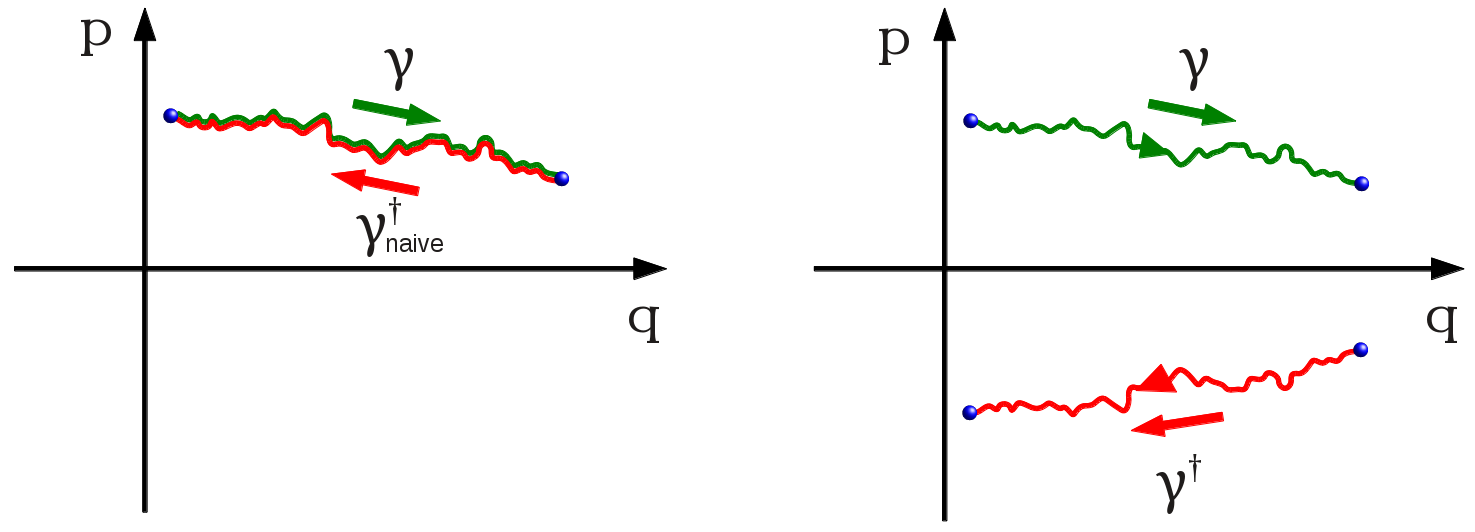
\includegraphics[width=26em]{reversal.png}
		\vspace{-1em}
	\end{figure}
	\begin{itemize}
		\item Time reversal in the Hamiltonian formalism is equivalent to \(p\to -p\)
		\item Not all variables transform the same under \(t\to-t\) -- ``odd and even variables'' need to be distinguished:
			\Align{
				\gamma = \{q(t),p(t)\} \longrightarrow \gamma^\dagger = \{\varepsilon q(T-t),\varepsilon p(T-t)\}
			}
	\end{itemize}
\end{frame}

\begin{frame}
	\frametitle{From the equations of motion to entropy}

	Rewrite the equations of motion to the corresponding Fokker-Planck equation
	\Align{
		\dot P(x,t) = -\sum_i\partial_i\underbrace{(A_i(x,t)P(x,t)-\partial_i(D_i(x,t)P(x,t)))}_{J(x,t)} \\
		\text{where } x = (q, p)
	}
	From this, the Green's function/short-time propagator \(G_a(\vec x'|\vec x\;;\mathrm dt)\) can be calculated, which \ldots
	\begin{itemize}
		\item solves the FP equation to lowest order in \(\mathrm dt\)
		\item is not unique, represented by the index \(a\) (similar to the It\={o}-Stratonovich dichotomy)
		\item Repeated application (convolution) yields the full propagagor
	\end{itemize}

\end{frame}

\begin{frame}
	\frametitle{From equations of motion to entropy}

	After obtaining the (lengthy) expression for \(G_a(\vec x'|\vec x\;;\mathrm dt)\), the differential (short-term) entropy production is
	\Align{
		\mathrm dS_\text{env}(\vec x'|\vec x;\;\mathrm dt) = \ln\frac{G_a(\vec x'|\vec x;\;\mathrm dt)}{G_b(\vec x'^\dagger|\vec x^\dagger;\;\mathrm dt)}
	}
	In the Spinney/Ford case (mirror momenta on the reverse path), this becomes
	\Align{
		\mathrm dS_\text{env}(q',p'|q,p;\;\mathrm dt) = \ln\frac{G_a(q',p'|q,p;\;\mathrm dt)}{G_b(q,-p|q',-p';\;\mathrm dt)}
	}
	Furthermore, Spinney/Ford show that \(a=1-b\) is the right choice of parameters, which cancels them both out.
\end{frame}

\begin{frame}
	\frametitle{Spinney/Ford differential entropy production}
	Using this approach, we showed that the Spinney/Ford approach for the simplest case of constant \(\gamma(p),\Gamma(p)\) yields
	\Align{
		\mathrm dS_\text{env} = -\beta p\mathrm dp - \gamma \mathrm dt
	}
	This seems very implausible, as a resting particle (\(p=0\)) produces negative entropy over time. This peculiar property of Spinney/Ford's approach motivated our research.
\end{frame}

\begin{frame}
	\frametitle{How to solve the problem?}
	\begin{itemize}
		\item Deterministic systems should not produce entropy.
		\item Jumping to another state should produce environmental entropy.
		\item Entropy production should be local, and not require jumping to another region of phase space entirely.
	\end{itemize}
	\underline{Idea:} What consitutes the ``state'' of a stochastic system? Could it be more than just a point in phase space?

	\underline{Proposition:} Identify the whole Hamiltonian trajectory as ``the state'' of a system. Switching trajectories produces entropy, staying on it doesn't.
\end{frame}


\begin{frame}
	\frametitle{A new way of reversing paths}
	Can we redefine the path reversal to solve these issues?
	\begin{figure}[htb]
		\vspace{-1em}
		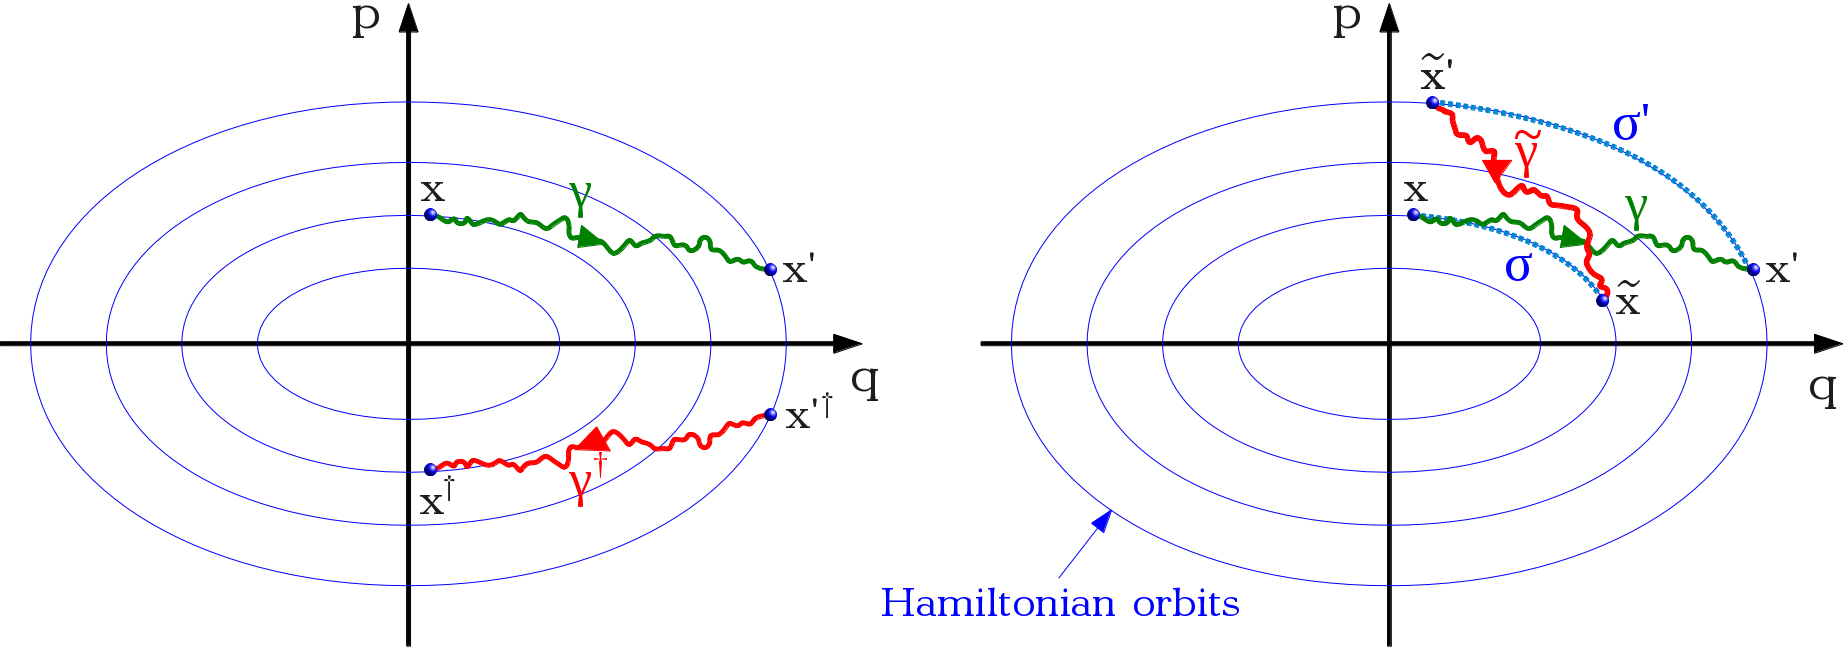
\includegraphics[width=26em]{trajectories.png}
		\vspace{-1em}
	\end{figure}
	\begin{itemize}
		\item Forward trajectory stays the same as in Spinney/Ford
		\item Backward trajectory: Instead of reversing the path, consider how likely the reverse transition between orbits (instead of points) would have been
	\end{itemize}

\end{frame}


\begin{frame}
	\frametitle{A new way of reversing paths}

	In formulas, this idea reads
	\Align{
		&\mathrm dS_\text{env}(q',p'|q,p;\;\mathrm dt) = \\
		&\qquad\ln\frac{G_a(q',p'|q,p;\;\mathrm dt)}{G_b(q+p\mathrm dt,p+f(q)\mathrm dt|q'-p'\mathrm dt,p'-f(q')\mathrm dt;\;\mathrm dt)}
	}
	Result for \(\mathrm dS_\text{env}\):
	\begin{itemize}
		\item Vanishes along the Hamiltonian flow (i.e. deterministic trajectories)
		\item \(a = b = \frac12\) turns out to be the right choice of parameters for the propagator ambiguity
	\end{itemize}
	
\end{frame}



\begin{frame}
	\frametitle{Comparing the models}

	\emph{Differential} entropy production \(\mathrm dS_\text{env}\) is not observable, the expected (average) entropy production however is. What difference do the models make in the result?

	\Align{
		\dot S_\text{env}(x) = \lim_{\mathrm dt\to0}\frac1{\mathrm dt}
			\int_\Omega \mathrm dx'
			G_c(\vec x'|\vec x;\;\mathrm dt)
			\mathrm dS_\text{env}(\vec x'|\vec x;\;\mathrm dt)
	}
	\Align{
		\dot S_\text{env}(t) = 
			\int_\Omega \mathrm dx'
			P(x,t)
			\dot S_\text{env}(x)
	}

	Results:
	\begin{itemize}
		\item The (third) ambiguity parameter \(c\) does not appear in the result in lowest order
		\item Both Spinney/Ford and the Flow model result in the same results, although the differential entropies are different
	\end{itemize}


\end{frame}


\begin{frame}
	\frametitle{Example system}
	For a system obeying detailed balance (FP equation stationary):
	\Align{
		\mathrm dS_\text{env} = \begin{cases}
			-\beta p(\mathrm d p + V'(q)\mathrm dt) {\color{red}- \frac\beta2\Gamma(p)^2\mathrm dt}
				& \text{Spinney/Ford}
				\\
			-\beta p(\mathrm d p + V'(q)\mathrm dt)
				& \text{Our model}
			\end{cases}
	}
	Because of the {\color{red}red term}, only our result vanishes along the deterministic trajectory \(\dot p = -V'(q)\). However,
	\Align{
		\dot S_\text{env} = -\frac12\Gamma(p)^2 + \frac23\beta^2p^2\Gamma(p)^2-\beta p\Gamma(p)\Gamma'(p)
	}
	is identical in both cases, as is the equilibrium entropy production,
	\Align{
		\langle\dot S_\text{env}\rangle_\text{DB} = \int_\Omega \mathrm dp \mathrm dq \frac{e^{-\beta(\frac{p^2}2-V(q))}}Z \dot S_\text{env}(q,p) = 0
	}
	which is the desired result, as a system obeying detailed balance should not produce entropy in the environment.

	
\end{frame}


\begin{frame}
	\frametitle{Conclusion}

	\begin{itemize}
		\item Spinney/Ford's differential entropy production shows odd behaviour in some cases
		\item Redefining the ``backwards'' path solves this issue, taking the non-stochastic Hamiltonian flow into accounthttps://news.ycombinator.com/item?id=5977495
		\item Both approaches yield the same physical quantity \(\dot S_\text{env}\)
	\end{itemize}

\end{frame}



\begin{frame}
	\begin{center}Thanks for your attention!\end{center}
\end{frame}









\end{document}


